% IEEE Paper Template for US-LETTER Page Size (V1)
% Sample Conference Paper using IEEE LaTeX style file for US-LETTER pagesize.
% Copyright (C) 2006 Causal Productions Pty Ltd.
% Permission is granted to distribute and revise this file provided that
% this header remains intact.
%
\documentclass[10pt,conference,letterpaper]{IEEEtran}
\usepackage{times,amsmath,epsfig}
\usepackage{subfigure}
\usepackage[margin=1in]{geometry}
%\usepackage{pgfplots}
\usepackage{color}
\usepackage{url}
\usepackage{hyperref}
\usepackage{multirow}

\newcommand{\todo}[1]{%                                                          
  \noindent {\bf {\color {red} TODO: #1 }}%                                      
}
\newcommand{\WW}[1]{%                                                          
  \noindent {\bf {\color {blue} #1}}%                                      
}

\usepackage{subfigure}
\pagenumbering{arabic}

\title{Energy Tuning of Polyhedral Kernels on Multicore and Many-Core Architectures}


% a short form should be given in case it is too long for the running head

%\titlerunning{Social Network Analysis on SQL Queries}
%\author{\IEEEauthorblockN{Wei Wang, William Killian, EunJung Park, John Cavazos}
%\IEEEauthorblockA{Department of Computer and Information Sciences\\
%University of Delaware\\
%Newark, DE 19716\\
%Email: \{weiwang,killian,ejpark,cavazos\}@udel.edu}
%}
\author{}


\begin{document}
\maketitle


\begin{abstract}
As the HPC community moves into the exascale computing era, application energy 
has become a big concern. Tuning for energy will be 
essential for the embedded systems to meet. in the effort to overcome the limited power envelope. How is 
tuning for lower energy related to tuning for faster execution? 
Understanding that relationship can guide both performance and energy tuning
for exascale. In this paper, a strong correlation is presented between the
two that allows tuning for execution to be used as a proxy for 
energy tuning.  We also show that polyhedral compilers can effectively tune a realistic application 
for both time and energy.

For a large number of variants of the Polybench programs and LULESH energy consumption is strongly correlated with total execution time.
Optimizations can increase the power and energy required between variants, but variant with minimum execution time
also has the lowest energy usage.
The polyhedral framework was also used to optimize a 2D cardiac wave propagation simulation application.
Various loop optimizations including fusion, tiling, 
vectorization, and auto-parallelization, achieved a $20\%$ speedup over the 
baseline OpenMP implementation, with an equivalent reduction in energy 
on an Intel Sandy Bridge system. On an Intel Xeon Phi system, improvements
as high as 21\% in execution time and 19\% reduction in energy are obtained.

\end{abstract}


\section{Introduction}
\label{sec:intro}
Reducing application energy consumption is important to improve user experience of 
embedded systems, e.g. smart phones, GPS navigators etc. 
Tuning applications for better energy efficiency is faced with challenges brought by
diverse architectures, difficulty of obtaining fine-grain measurements of power, 
as well as enormous amount of tuning choices.
This work uses the RCRtool \cite{us}, a fine-grain energy measurement tool, to easily attribute energy consumption to particular
regions of application kernels and to serve energy tuning. 
When tuning the application for
better execution time and energy usage, some combination of loop optimizations, including loop 
tiling, loop unrolling, and loop fusion, are usually performed on kernels along with the auto-parallelization.
Determining which set of optimizations produces the best results is hard.
Polyhedral auto-tuning frameworks have shown promising results at simplifying that effort\cite{EJ2012}
for small computation kernels like the Polybench programs. 
This work investigates the effectiveness of such framework to tune for 
energy on two different multi-core architectures: Intel Sandy Bridge
and Many Integrated Core (MIC).
 
This paper has two main contributions: 
(1) Performance speedups and energy savings on Sandy Bridge and MIC for various Polybench kernels applying loop transformations. 
(2) Evaluation of architectural differences of energy behaviours corresponding to the same loop transformations.

The rest of the paper is organized as follows. In Section~\ref{sec:tools}, we describe the tools
used to measure energy consumptions. Section~\ref{sec:benchmarks} describes the benchmarks used for  
measuring the energy consumptions. Experimental results and analysis are presented in Section~\ref{sec:results}. Section~\ref{sec:conclusion} has our conclusions.



\section{Energy Measurement-and-Tuning Tools}
\label{sec:tools}
To understand energy consumption, execution time and various optimizations,
a light-weight fine-grained measurement tool is required. RCRtool provides 
user-level fast access to hardware counters.
Finding the optimal combination of compiler optimizations 
requires a compilation framework, like the Polyhedral Compiler
Collection, that easily produces a large number of 
program variants with specific optimization parameters.

The Intel Sandy Bridge architecture allows users to track energy usage through 
the exposed Running Average Power Limit (RAPL) interface\cite{IntelSystemProgrammingVol3}. 
A model-specific register (MSR) was added with the Sandy Bridge to track energy
consumed by the chip  -- MSR\_PKG\_ENERGY\_STATUS.
The counter is frequently updated and counts the energy in 15.3 micro-Joule units.
Experiments have shown\cite{us} and the documentation\cite{IntelSystemProgrammingVol3} states
that the counter can be accessed as often as every microsecond. 
The counter is only 32 bits and can wrap in as little as a couple of minutes.
The RCRtool detects the wraps and supplies a 64 bit value with the 
upper 32 bits being the number of wraps since RCRtool instantiation.
The RCRtool must run at supervisor level to access the counter.
It writes the current value of the counter at least 1000 times a second into a shared-memory
data structure. This ``blackboard'' structure provides a hierarchical view of the system
where various current performance information is stored. The 
information is available to any OpenMP applications through a simple API that 
delineates a code region for measurement with a start and end call.
Each region is identified by its file name and line number.
If a region is executed multiple times the energy is summed across all executions. 
All energy information is available during application shutdown.

When the program finishes execution,
the elapsed time, the amount of energy used (in Joules), and the average computed
power (in Watts) of the kernel regions and the whole application are output. 
RCRtool runs on Intel architecture with the RAPL interface, and has been tested
on Sandy Bridge and Ivy Bridge implementations.

The overhead of the RCRdaemon is negligible on both architectures.  
It enables us to measure the energy consumption of the application 
with a granularity of about one millisecond. 

\subsection{RCRtool on Xeon Phi System}
The Intel MIC architecture in the Intel Xeon Phi chips is a recent addition to the
Intel processor offerings.
Our Phi accelerator cards contain 61 cores, each core supports 4 hardware threads. 
One notable feature is the 512-bit wide SIMD vectors providing fine-grain
vectorization and high floating-point performance for each thread.
With the wide vector registers, a single 
instruction can operate on 8 adjacent double-precision floating point data or 16 
single-precision floating point data. The cores, threads and vector unit combine
to achieve well over a Teraflop from a single socket.

RCRtool collects power information of Intel Phi natively
or on the host. Natively, users can track power usage in microWatts through    
a file (/sys/class/micras/power) updated every 50 millisecond.
RCRtool monitors the power at user level and computes the energy
consumption over time.
The information is available to the applications through the same simple API as on
Sandy Bridge.

RCRtool can also run on the host. On the host, it collects
power information using the MICAccessSDK API provided by Intel at the same 
granularity as the native version. 
Measurements in this paper were collected with a native Phi RCRdaemon.
 
\subsection{Polyhedral Optimizations Tools}
The Polyhedral Compiler Collection (PoCC)\cite{PoCC} was used to generate program 
variants with different optimizations.
The PoCC requires that programs contain static control parts (SCoP)\cite{SCoP1,SCoP2} so that 
valid transformations can be applied. Polybench is a collection of programs
that contain SCoPs and can be polyhedral optimized.  
PoCC generates hundreds and even thousands of program variants for simple programs, like Polybench.


\section{Benchmarks for Energy Measurement and Tuning}
\label{sec:benchmarks}
In this work, we evaluate three kinds of programs for energy auto-tuning with
polyhedral framework: Polybench programs, publicly-accessible LULESH 
program\cite{LULESH:versions}, and a realistic application developed and frequently 
used by our collaborators.

\subsection{Polybench}
Previous work has obtained significant speedups with the 
polyhedral framework for the Polybench programs\cite{EJ2011,EJ2012,EJ2013}.
Extending that work to examine whether the best tuned variants are also
the most energy efficient is the focus of this work.
Using PoCC, program variants were generated using
a different set of the 
optimizations from the following five groups: 
\begin{itemize}
    \item Loop fusion: smartfuse, maxfuse, nofuse
    \item Loop unrolling factor: 1, 2, 4, 8
    \item Loop tiling: 1, 16, 32, 64. Note that the number of different flags
 depends on the level of nested loops   
    \item Loop vectorization: on, off
    \item Loop parallelization: on, off
\end{itemize}
%\WW{We rely on Tiling Hyperplane method\cite{Hyperplane} to legally perform loop
%transformations. Loop fusion is performed to maximize locality by fusing statements. 
%As in\cite{EJ2013}, 1) nofuse means we do not fuse statements at all;
% 2)smartfuse means we only fuse together statements that carry data reuse and of 
%similar loop nesting depth; 3) maxfuse means we maximally fuse statements.
% }
The Tiling Hyperplane method\cite{Hyperplane} is used to legally perform loop transformations.
Loop fusion is performed to minimize loop overheads. Depending on reuse patterns, fusion can increase or decrease locality. As in\cite{EJ2013}, 1) nofuse results in no loop fusion 2) smartfuse only
fuses statements that carry data reuse and are at similar nesting levels 3) maxfuse performs all legal loop fusion.
If the maximum nested loop level is 3, applying all possible combinations
of the above flags generates 5135 program variants. The ROSE source-to-source
compiler was used to add energy profiling calls to each variant.
GCC(4.4.6) generated the final executable. During execution,
 periodic queries to the RCRtool blackboard provide the energy consumption information.
Figure~\ref{fig:Workflow} gives the workflow for measuring energy consumption of 
Polybench programs using the energy-aware polyhedral compiler framework.

\begin{figure}[t]
    %\rotatebox{-90}{\includegraphics[height=3in]{TE}}
    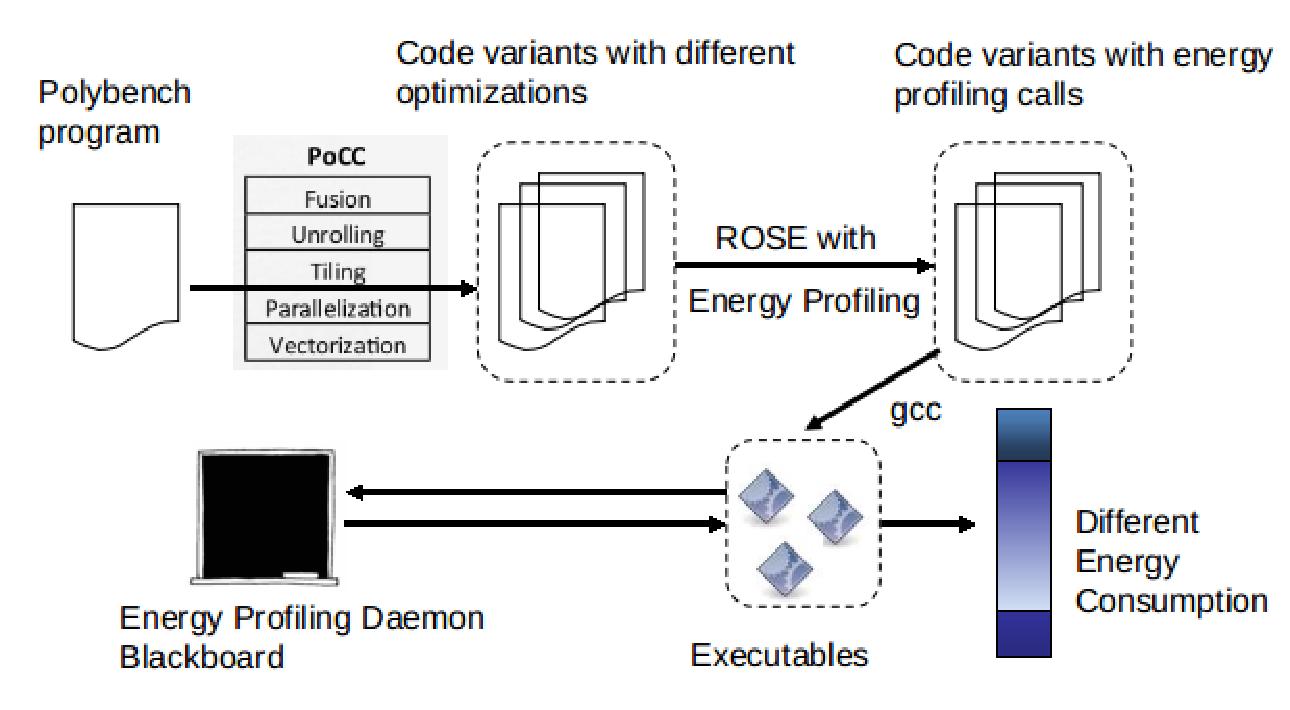
\includegraphics[width=3.4in]{workflow}
    \caption{Graph showing the workflow of obtaining energy consumption of polyhedral
optimized (Polybench) programs. }
    \label{fig:Workflow}
\end{figure}

\subsection{LULESH}
LULESH\cite{LULESH:versions} is a shock hydrodynamic simulation application. It
mimics a larger realistic application called ALE3D. We used the OpenMP implementation
v1.0 for evaluation. The original LULESH uses a 
block structured mesh accessed via an indirect reference pattern\cite{LULESH:versions}.
%In order to make LULESH go through the polyhedral compilation procedure, we modified
To make LULESH go through the polyhedral compilation procedure, we modified
LULESH by resolving all indirect array accesses. Although doing this oversimplified
LULESH, it allows us to study the energy and time relationship of polyhedral 
compilation techniques with LULESH. 

LULESH OpenMP implementation contains 30 parallel regions, 6 of which take up more
than $60\%$ of the total application time\cite{us}. We manually converted two most 
significant parallel regions to two SCoPs so that they can be passed to polyhedral
framework. The resulting largest SCoP contained too many dependences and we found
it was hard for the polyhedral compiler to finish transformation and parallelization.
When all temporary variables were eliminated from the most computationally intensive loop
to create an SCoP, greatly expanded statements required hours of compilation to finish generating even one variant.
%Even when all the dependences are eliminated inside the largest SCoP, it still took the polyhedral
%compiler hours to finish one transformation.
In this work, we focus on optimizing 
the 2nd (largest) SCoP of LULESH. 200 program variants were produced 
by applying loop fusion (maxfuse and 
smartfuse), loop tiling, vectorization, and parallelization.
The execution time and energy of each was measured.

\subsection{A Realistic Application}
In addition to the Polybench programs, a 2D monodomain cardiac wave propagation simulation 
(named \emph{brdr2d}) was used as a test case. Its model involves
solving a set of ODEs and PDEs and is well-known in the computational 
cardiac modeling field\cite{Me}. Equation (1) is the PDE that needs to be 
solved. The ODEs are used to represent the $I_{ion}$ variable.
\begin{equation}
C_{m}\frac{\partial V_{m}}{\partial t} = \nabla \cdot D\nabla{V_{m}}-I_{ion}
\end{equation}
The sequential C implementation is more than 1K lines. 

One loop nest takes up more than 90\% of the total application execution time. 
The dominate loop nest is an ideal situation for the polyhedral compiler. 
The loop nest is inside a while loop and is executed many times. 
This code structure is not unique to cardiac wave propagation simulation. 
Computationally dominate loops inside either while loops looking for 
some termination condition or inside a simulation time-step loop
are common in scientific codes. LULESH falls into this category
with multiple loop nests within a time-step loop.

While PolyOpt originally cannot extract any SCoP from \emph{brdr2d}, it does output
information useful to the user to manually transform the application to contain at least one SCoP.
To expose the SCoPs the following changes were required. The computation part 
of \emph{brdr2d} was fully inlined removing all function calls.
Then, all array indexes were changed to be affine functions of the 
loop iterators. This involved loop unswitching to specialize modular operations
like $step~\%~2$. Finally, the number of dependencies was reduced by forward substitution
of temporary variables. After these changes, PolyOpt automatically detected the code
region and applied various transformations to the SCoPs. 

%Different from LULESH, the forward substitution did not result in 
%extreme expansion of code when converting the nested loops into SCoPs. Thus, the 
%polyhedral compiler generated program variants in a timely manner.

Program variants were generated to explore data locality and parallelism
using loop fusion (smartfuse/maxfuse), different tiling sizes, vectorization and auto-parallelization. 
OpenMP pragmas were automatically generated for each variant.
%The original sequential C implementation had OpenMP pragmas manually added to serve as
The original sequential C implementation had all required OpenMP pragmas manually added to serve as
a baseline.
Four different input files for \emph{brdr2d} were used to study how the
performance of the program variants is impacted by different
input sizes. 
 


%\section{Experimental Setup}
%\label{sec:setup}
%The tests ran on a machine with dual socket 8-core Intel Xeon E5-2680 processor with 20MB (40MB total) L3 cache.
The input graph is pnnl.bin, with which the whole application finishes in about 22 seconds.
It contains three (among many) most significant loops. Each of the loops takes about 3 seconds. 
%To protect against low start-up energy/power measurements, the system was warmed up
%with a computational intensive script before any test was executed.




\section{Experimental Results}
\label{sec:results}
First we report the speedups and energy saving achieved on two architectures applying
loop optimizations. Then we show loop optimizations that work the best on
one architecture do not necessarily work the best on the other, in terms of
time taken and energy consumed.
\subsection{Speedups and Energy Savings}

\begin{table}
  \centering{
\caption{Time and Energy Comparison of Optimal Configuration to Baseline of Polybench Kernels}
\begin{tabular}{ |l|c|c|c|c| }
  \hline
  \multirow{2}{*}{\textbf{Benchmark}} & \multicolumn{2}{|c|}{\textit{Time}} & \multicolumn{2}{|c|}{\textit{Energy}} \\
  \cline{2-5}
  & SM & LG & SM & LG \\
  \hline
  2mm & 1.48X & 1.36X & 1.28X & \textcolor{red}{0.77X} \\
  \hline
  covariance & 37.86X & 122.20X & 25.11X & 60.31X \\
  \hline
  gemm & 1.46X & 1.44X & 1.28X & \textcolor{red}{0.78X} \\
  \hline
  gramschmidt & 19.41X & 21.64X & 13.66X & 11.72X \\
  \hline
  jacobi-2d & 1.31X & 1.48X & 1.37X & 1.44X \\
  \hline
  seidel-2d & 7.76X & 9.60X & 7.68X & 5.53X \\
  \hline
\end{tabular}
}
\end{table}

\subsection{Cross Architecture Comparsion}

\begin{figure}
\centering
\subfigure[Best SandyBridge Optimization Sequences on Xeon Phi] {                        
  %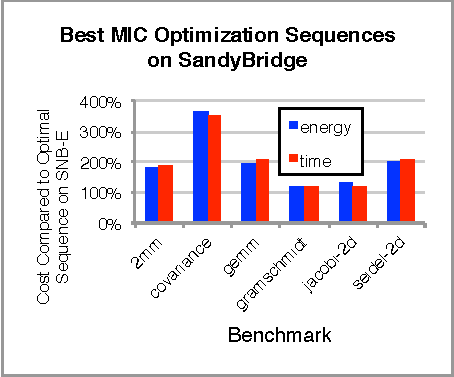
\includegraphics[width=0.45\textwidth]{BestMIConSNB}   
  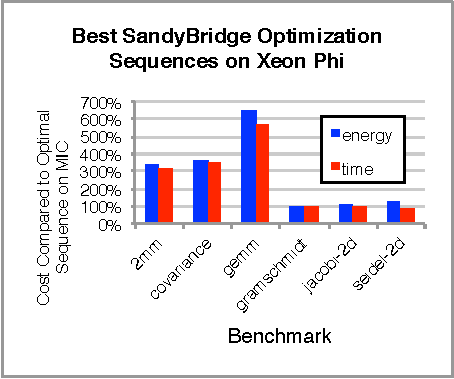
\includegraphics{BestSNBonMIC}
  \label{Sandy}
} 
\subfigure[Best MIC Optimization Sequences on SandyBridge] {               
  %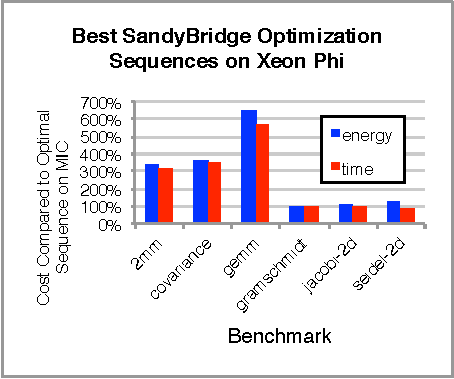
\includegraphics[width=0.45\textwidth]{BestSNBonMIC}
  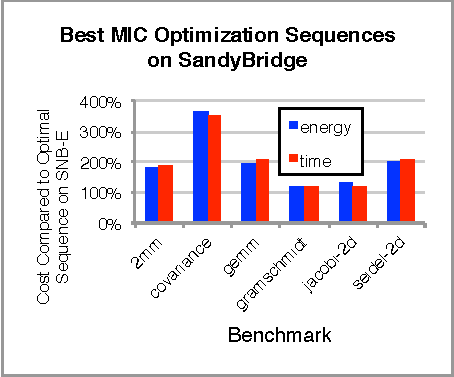
\includegraphics{BestMIConSNB}   
  \label{MIC}
} 
\caption{
}                   
\label{fig:Brdr2d-TE}                                                   
\end{figure} 

Figure~\ref{Sandy} shows the best optimization sequences of the six benchmarks
chosen from Sandy Bridge do not perform as good when run on the MIC architecture. 
Comparing with the optimal optimization sequence on the MIC, the Sandy Bridge
sequences incurred significant increase in execution time and energy consumption
for 2mm, covariance, and gemm. The Sandy Bridge optimization sequences 
performed as good as the optimal sequence on the MIC for the other three benchmarks. 
Figure~\ref{MIC} compares the time and energy (running on Sandy Bridge) of 
the best optimization sequences chosen from MIC with those of the optimal optimization 
sequences chosen from Sandy Bridge. 2mm, covariance, gemm, and seidel-2d consumed
from ~200\% to ~350\% more energy and time. 


%\section{Related Work}
%\label{sec:related}
%%\todo{Needs work to make sense}
\subsection{Benchmarks for Polyhedral Framework and Auto-parallelization}
There are a few benchmarks available to evaluate polyhedral transformations as 
an approach to improving application performance.  Our work adds two non-trivial application (LULESH and \emph{brdr2d})
to the family of benchmarks that are polyhedral optimizable. Polybench\cite{Polybench} and 
SWIM\cite{SWIM} benchmark are two benchmark suites that are often used. The Polybench programs evaluate polyhedral 
transformations and are used to construct predictive models by Park {\it et al.}\cite{EJ2011,EJ2012, EJ2013}.
They are also used to evaluate auto-parallelization techniques targeting different architectures,
using different tools. Grauer-Gray {\it et al.}\cite{Scott} utilized high level languages 
to target GPU architecture by annotating Polybench programs. Konstantinidis {\it et al.}\cite{LCPC2013}
studied GPU code generation given the Polybench programs that contain affine loops. 
%Our cardiac wave propagation simulation benchmark can help the design and evaluation of new
%techniques.
 
\subsection{Tuning for Performance and Energy}
Rahman {\it et al.}\cite{CF12} studied the impact of application level optimizations from both the 
performance and power efficiency perspective of various applications. They found
that optimizing for performance did not guarantee better power consumption. We 
observed similar results in Figure~\ref{fig:TE} and Figure~\ref{fig:2mm-TE} for non-optimal
program variants but the graphs showed that for the optimal case, tuning for performance and power were 
effectively equivalent. To improve performance and energy efficiency for a Many-Core architecture,
Garcia {\it et al.}\cite{Garcia} studied the energy consumptions of applications and proposed models 
characterizing application energy consumption footprints. We did not
develop energy models but took advantage of the exposed hardware interfaces to obtain accurate   
energy consumption information from modern commodity processor architectures like
Intel Sandy Bridge and Xeon Phi.

To improve performance, people have 
developed techniques from distinctive ways. Tavarageri {\it et al.}\cite{Reduce-Cache} 
adopted compiler analysis approach to configure the cache size to reduce energy consumption
without performance loss. New programming languages\cite{IPDPS13:LULESH} and 
models like Chapel, Liszt and others were introduced to facilitate program optimizations
on parallel architectures.


\section {Conclusion}
\label{sec:conclusion}
In this work, we tuned six representative Polybench kernels for energy on
an Intel SandyBridge processor and an Intel Xeon Phi coprocessor by applying various loop 
transformations. For the \texttt{2mm} and \texttt{gemm} kernels (dense matrix kernels),
we observed \emph{non-correlated} speedups and energy savings over the baseline version,
i.e. \emph{fastest execution does not guarantee fewest energy consumption}. 
We also showed that good loop transformations for one architecture do not carry over to
other architectures.


%\balancecolumns

%ACKNOWLEDGMENTS are optional
%\section{Acknowledgments}
%This work is supported by the DOE XPress (DE-SC0008704) and the DoD ATPAR (PNNL-214990).

\bibliographystyle{IEEEtran}

\bibliography{SEAK}  % sigproc.bib is the name of the Bibliography in this case



\end{document}
